\documentclass[9pt,twocolumn,twoside]{g3_article/gsag3jnl}

% Packages.

\usepackage{multirow}
\usepackage{caption}
\usepackage{tikz}

\articletype{gs} % article type
% {inv} Investigations
% {msr} Mutant Screen Reports
% {gs} Genomic Selection
% {goi} Genetics of Immunity 
% {gos} Genetics of Sex 
% {mp} Multiparental Populations

\title{Genomic Selection with Deep Neural Networks}

\author[$\ast$,1]{Riley McDowell}
\author[$\dagger$]{David Grant}
%\author[$\ddagger$]{Author Three}
%\author[$\S$]{Author Four}
%\author[$\ast\ast$]{Author Five}

\affil[$\ast$]{Iowa State University, US}
\affil[$\dagger$]{Iowa State University, US}
%\affil[$\ddagger$]{Author three affiliation}
%\affil[$\S$]{Author four affiliation}
%\affil[$\ast\ast$]{Author five affiliation}

%For the authors' names, indicate different affiliations with the 
%symbols: $\ast$, $\dagger$, $\ddagger$, $\S$. After four authors
%, the symbols double, triple, quadruple, and so forth as required.

\keywords{ genomic prediction \\ deep learning \\ neural network \\ genomic selection \\ SNP }

\runningtitle{ Genomic Selection with Deep Neural Networks } % Goes into the footer.

\correspondingauthor{Corresponding Author HERE} % TODO: Who is this?

Reduced costs for DNA marker technology coupled has generated a huge amount of
molecular data and greatly increased the options available to characterize lines 
in a breeding program. Concurrently, the field of machine learning has experienced
a resurgence of research into techniques to detect or "learn" patterns in noisy
data in a variety of technical applications. Here, we apply so called "deep learning"
techniques from current machine learning research related to neural networks to five 
genomic selection and phenotypic selection problems using published reference datasets. 
We compare the results of these algorithms to a selection of bayesian and linear 
regression techniques commonly employed today. TODO: FINDINGS/RESULTS/CONCLUSIONS.


%The abstract should be written for people who may not read the 
%entire paper, so it must stand on its own.  The impression it makes usually determines 
%whether the reader will go on to read the article, so the abstract must be 
%engaging, clear, and concise.  In addition, the abstract may be the only part of the 
%article that is indexed in databases, so it must accurately reflect the 
%content of the article. A well-written abstract is the  most effective way to reach intended 
%readers, leading to more robust search, retrieval, and usage of the article. 
%
%Please see additional guidelines notes on preparing your abstract below.

%\begin{itemize}
%\item provide a synopsis of the entire article;
%\item begin with the broad context of the study, followed by specific background for the study;
%\item describe the purpose, methods and procedures, core findings and results, and conclusions of the study;
%\item emphasize new or important aspects of the research;
%\item engage the broad readership of G3 and be understandable to a diverse audience (avoid using jargon);
%\item be a single paragraph of less than 250 words;
%\item contain the full name of the organism studied;
%\item NOT contain citations or abbreviations.
%\end{itemize}



\setboolean{displaycopyright}{true}

\begin{document}

\maketitle
\thispagestyle{firststyle}
\logomark
\articletypemark
\marginmark
\firstpagefootnote
\correspondingauthoraffiliation{TODO: CORRESPONDING AUTHOR ADDRESS AND EMAIL HERE}
\vspace{-11pt}

\noindent % Skip header for 'Introduction'.


The wide availability and reduced cost of molecular marker technology
has created opportunities to perform marker assisted selection of genotypes
in plant and animal breeding. Quantitative Trait Locus (QTL) mapping techniques
have proved useful for identifying markers genetically associated with genes 
conditioning agronomic phenotypes \citep{miles2008}. Using identified QTL to
support selection has grown in popularity as molecular marker data costs have 
decreased. Once a sufficient proportion of QTL-associated markers have been identified, 
the associated markers can be leveraged for making selections on a population. 
Individuals in a population genotyped for previously identified QTL-associated
markers can be selected based on the presence of desired alleles 
and/or haplotypes in a process known as Marker Assisted Selection (MAS).
MAS is usually effective on traits with a few large effect alleles with high 
heritability. However, when making selections on traits with many contributing genes 
with small effect distributed widely across a genome, MAS becomes less 
effective \citep{heffner2009}.

In order to apply MAS to traits with diverse genetic architectures, it is
advisable to combine MAS on juvenile individuals and subsequent phenotypic
selection on adults with favorable MAS scores \citep{lande1990}. This process, 
known as two-stage selection, has proven effective for improving
the coefficient of selection of breeding programs while avoiding expensive phenotypic
trials for individuals with low genetic potential. While inexpensive, two-stage selection 
only utilizes those markers associated with QTL with significant effects. The present cost of
genome wide SNP assays has fallen dramatically enough that today individuals are
frequently genotyped for hundreds, thousands, or even tens of thousands of SNPs. 
Information in SNPs that are not significantly associated with a trait are lost 
when applying MAS and two-stage selection, but may still have an small effect on the
expressed phenotype and thus could provide improved predictive 
accuracy of individual's genetic value.

Unlike QTL mapping and associated MAS techniques, genomic prediction methods
attempt to predict phenotypes utilizing all available SNP marker data collected 
from a population, allowing one of many possible statistical models to predict 
the marker-trait associations in a data driven way \citep{meuwissen2001}. 
The accuracy of genomic prediction relies on an appropriate choice of a 
statistical model to capture the relationship between the genetic architecture
of a trait and the underlying marker calls in a panel of high-density marker 
data. It is likely that the best statistical model for genomic prediction is 
dependent on the genetic architecture of
the predicted trait \citep{crossa2010, gonzalez-camacho2012, 
resende2012, cleveland2012, thavamanikumar2015}.  From a mathematical perspective,
models incorporating interactions between marker features have the 
capacity to achieve higher accuracy by capturing non-additive effects.
Experimental results support this hypothesis \citep{gonzalez-camacho2012}. 
Alternative prediction methods continue to be an active area of research 
in plant and animal breeding \citep{koning2012}.

% A more rapid transition into information about neural networks
% than is present in the lit review. This skips sections 
% describing selecting a particular model and of the fields of data science.
Concurrent with the advent of genomic selection as a practice the popularity of the 
interdisciplinary field known as data science has increased. Practitioners of data 
science apply machine learning and statistics to make predictions, usually
by applying ideas or techniques from a wide variety of domains 
including mathematics, physics, and computer science. Often, a data scientist's focus is to
create a predictive model than may not be associated with an underlying generative model. 
This can be viewed as the distinction between data science and classical statistics 
\citep{donoho2015, breiman2001}. The rapid increase in popularity of data science
is associated with better definitions of best practices for predictive modeling
across many disciplines as well as software packages to automate the 
process of building predictive models from any data source.

Neural networks are a type of model frequently employed by data scientists
for predictive modeling. Neural networks consist of layers of interconnected neurons
which map inputs to one or more outputs. Each neuron in a network can be expressed as a 
transformation of a weighted sum of $n$ inputs 

\begin{equation}
output_{lk} = \sum_{i=1}^{n} f_l(w_{lki} * x_{i} + b_{lk})
\label{eq:neuron}
\end{equation}

where $output_{lk}$ is the output from neuron $k$ in network layer $l$ having activation
function $f_l$, weights $w_{lki}$ and bias $b_{lk}$.

A neural network is a collection of neurons that map a 
length $n$ input vector $x = (x_1, ..., x_n)$ through a series of $j$ 
"hidden" layers $(l_1, ..., l_j)$. Each hidden layer consists of a variable 
number of neurons, each of which apply an associated coefficient, bias, and 
mathematical transformation to their input and forward the 
result on to every neuron in the subsequent layer forming an interconnected
network (Figure \ref{fig:deepnet}).

\ifdefined\showtablesandfigures
% A deep neural network with 3 hidden layers of varying sizes.

\begin{figure}[htbp]
\renewcommand{\familydefault}{\sfdefault}\normalfont
\centering

\def\layersep{1.5cm}

\begin{tikzpicture}[shorten >=1pt, ->, draw=black!50, node distance=\layersep]
    \tikzstyle{every pin edge}=[<-, shorten <=1pt]

    \tikzstyle{neuron}=[circle, fill=black!25,minimum size=17pt, inner sep=0pt]
    \tikzstyle{input neuron}=[neuron];
    \tikzstyle{output neuron}=[neuron];
    \tikzstyle{hidden neuron}=[neuron];

    \tikzstyle{annot}=[text width=4em, text centered]

    \foreach \name / \y in {1,...,5}
        \node[input neuron, pin=left:Marker \#\y] (I-\name) at (0,-\y) {};

    \foreach \name / \y in {1,...,4}
        \path[yshift=-0.5cm]
            node[hidden neuron] (H1-\name) at (\layersep * 1,-\y cm) {};

    \foreach \name / \y in {1,...,5}
        \path[yshift=0.0cm]
            node[hidden neuron] (H2-\name) at (\layersep * 2,-\y cm) {};

    \node[output neuron, pin={[pin edge={->}]right:\small{Prediction}}, right of=H2-3] (out) {};

    \foreach \source in {1,...,5}
        \foreach \dest in {1,...,4}
            \path (I-\source) edge (H1-\dest);

    \foreach \source in {1,...,4}
        \foreach \dest in {1,...,5}
            \path (H1-\source) edge (H2-\dest);

    \foreach \source in {1,...,5}
        \path (H2-\source) edge (out);

    \node[annot, above of=I-1, node distance=1cm] (il) {\small Input Layer};
    \node[annot, right of=il] (hl1) {\small Hidden Layer 1};
    \node[annot, right of=hl1] (hl2) {\small Hidden Layer 2};
    \node[annot, right of=hl2] {\small Output Layer};
\end{tikzpicture}

\caption{A deep feedforward neural network. Many input marker calls are mapped 
         to one or more sequential hidden layers of neurons. For genomic selection, the
         input layer often consists of one neuron per marker and the output consists of a single
         neuron which combines the information from the final hidden layer to predict a phenotype or BLUP.
         The presence of more than one hidden layer indicates that a network is likely to learn
         higher order non-linear interactions, and can be called a deep network.}
\label{fig:deepnet}
\end{figure}
 % Label = fig:deepnet
\fi

Once the network is defined, it must be exposed to input and desired output
values, and adjusted to minimize error in output in a process known as training.
The weights and biases are often initialized by drawing from a
random normal distribution. From this initial state, error in 
the output of the network is propagated back through the hidden 
layers, and the weights and biases are updated in the direction that would 
decrease output error on many randomly drawn subsets of the input data. 
This turns the network training process into a general 
function minimization problem, where the parameters to the function are the 
weights and biases of the network neurons and the function to be 
minimized is the squared differences between the network outputs and 
the desired true values. The process of propagating output error back 
through a neural network is known as backpropagation, and has been used 
and improved extensively since its original description in the 
1980s \citep{rumelhart1986}.  Typically, the training data is split 
evenly into representative, randomly sampled collections of data 
called batches. The training algorithm exposes the network to each 
batch until they are depleted, after which the process is repeated. Each 
collection of batches is known as an epoch, and training typically
involves applying backpropagation for several hundred epochs, or until the network
weights and biases reach an equilibrium state that has converged to a 
globally minimum amount of prediction error.

%Good post, good links to the 'deep' part of deep nets.
%http://stats.stackexchange.com/questions/182734/what-is-the-difference-between-a-neural-network-and-a-deep-neural-network

It is trivial to add additional hidden layers to an existing neural network model.
Despite the ease of describing their architecture, networks with many hidden 
layers have been notoriously difficult to train. The amount of error
attributed to a neuron by backpropagation decreases in magnitude with each
additional layer added to the network. As a result, layers nearest the input train
very slowly in a phenomenon known as the vanishing gradient problem \citep{hochreiter1998}. 
Recently, a series of breakthroughs in neural network training along with well-known
increases in computer processing speeds have allowed efficient training
of deeper networks than were previously possible \citep{sutskever2013}.
A history of the deep learning literature is available in \cite{lecun2015}.
The increased training efficiency and potential to capture subtle
correlation relationships between two or more input features drove a need to 
differentiate these deeper networks from prior work, resulting in 
the emergence of the phrase "deep learning" to describe the construction 
and training of deep neural networks.

Previous attempts to apply neural networks to genomic prediction have resulted in 
an overfitting of the network to the training data and raised 
concerns about the computation time required to fit the model to datasets containing
many markers across many genotypes \citep{heslot2012, gonzalez-recio2014}. 
In retrospect, these results are not surprising. Multi-layer feedforward neural networks 
are capable of approximating functions of arbitrary complexity to arbitrary 
accuracy if provided enough neurons in even a single hidden 
layer. This property of neural networks is known as the 
universal approximation theorem, and can result in
overfitting if the weights of the network are not regularized in some way \citep{hornik1989}.

Given the promising results from regularized and Bayesian methods for
genomic prediction such as ridge or LASSO regression and the Bayesian family of regressors,
it is prudent to evaluate some of the many of neural network training algorithms which
incorporate regularization of weights during training. Today, networks based on these
and other regularization techniques continue to show success
across many domains \citep{schmidhuber2015}. Similarly, while neural networks are 
computationally demanding to train, the training algorithms 
themselves are often easily expressed with vector and matrix algebra. These algorithms are 
well suited to execution on Graphics Processing Unit (GPU) hardware, with reports 
of up to a sixty-fold speedup in training time \citep{sierra2010, schmidhuber2015}. 

To facilitate the evaluation of regularized neural networks, a neural 
network prediction model was implemented supporting two regularization
techniques. The first is a weight decay regularization which penalizes the 
weights $W$ with very large values similar to ridge regression \citep{krogh1992}.
The second is dropout regularization, in which a portion of neurons and 
their connections are removed at random during each training epoch, 
encouraging subsets of the network to learn to recognize input features 
independently. This allows neurons to adapt and build independently 
operating units, preventing the neurons from co-adapting and reducing 
overfitting \citep{srivastava2014}. In order to support training deep networks, 
network weights were initialized in a way that is known to cause
deep networks to converge to a global minimum error more rapidly \citep{glorot2010}. 
A modified form of backpropagation designed for deep network training 
was also selected \citep{dozat2015}. Finally, a divergence detection method and 
learning rate decay method were implemented to ensure models converged to
a global minimum error.

In this paper, we present the results of using this deep neural network
configuration to perform genomic prediction on three benchmark datasets 
from different species. A high and low heritability trait was selected 
from each dataset for a total of six genomic prediction tasks. A collection 
of regression techniques including single hidden layer and deep neural networks were 
applied to each task. We also quantitatively evaluate the 
time required to train neural networks using both CPU and GPU based 
network fitting. Last, we compare the performance of the regularized network
implementation with other available genomic prediction models in the collection.

% For the introduction, authors should be mindful of the broad readership of the journal.
% The introduction should set the stage for the importance of the work to a generalist 
% reader and draw the reader in to the specific study. The scope and impact of the 
% work should be clearly stated.



\section*{Materials and Methods}

Five benchmark datasets of paired phenotypic and genotypic marker data were predicted 
using a collection of regression techniques. Benchmark species included three food crops, 
one forestry species, and one animal species. Benchmark traits include a variety of high and low
heritability traits with simple and complex genetic archetectures. Each dataset was divided
into 10 partitions by drawing entries without replacement and predicted with each
regression technique using ten-fold cross validation. The partitions of the data were 
held constant across all regression techniques to facilitate a fair comparision of the
prediction accuracy of each technique.

For statistical models with tunable hyperparameters, a grid-search of the parameter 
space was conducted and the parameters that produced maximum accuracy on the hold-out
data folds are used in the final analysis. 

The full analysis pipeline, including formatted datasets, quality control processes, 
implementations of each model, and final hyperparameter settings are available in File S1 *TODO* and
in a public repository on github \citep{mcdowell2016}.

%Manuscripts submitted to G3 should contain a clear description of the experimental design in sufficient detail so that 
%the experimental analysis could be repeated by another scientist. If the level of detail necessary to explain the 
%protocol goes beyond two paragraphs, give a short description in the main body of the paper and prepare a detailed 
%description for supporting information.  For example, details would include indicating how many individuals were used, 
%and if applicable how individuals or groups were combined for analysis. If working with mutants indicate how 
%many independent mutants were isolated. If working with populations indicate how samples were collected 
%and whether they were random with respect to the target population.

\subsection*{Statistical Analysis} 

Least squares, ridge, lasso, and elastic net regression were applied as examples of
linear regression with and without normalization penalties. Bayesian 
ridge regression is a bayesian version of ridge regression that assumes that 
the residual error in the model is gaussian distributed. These five regression 
techniques are implemented in the scikit-learn python package version 0.17.1 \citep{scikit-learn}.

A single parameterized neural network with dropout and weight-decay parameters was built using 
the Keras modular neural network library \citep{chollet2015}. The neural network results presented in this
manuscript were trained and evaluated using the default Theano backend \citep{team2016}. 
All training was conducted on an NVIDIA GTX 680 graphics card with 4GB 
of RAM using the CUDA 7.5 toolkit \citep{nickolls2008}. A network with no regularization,
as well as with one or both of the weight-decay and dropout regularization parameters
supplied was trained on each dataset. A summary of all regression methods is presented in Table \ref{tab:regression-methods}.

\begin{table*}[htbp]
\renewcommand{\familydefault}{\sfdefault}\normalfont
\centering
\caption{\bf Regression Methods}

\begin{tableminipage}{\textwidth}

% Benchmark Datasets table.

\begin{table*}[htbp]
    \renewcommand{\familydefault}{\sfdefault}\normalfont
    \centering
    \caption{\bf Regression Methods}

    \begin{tableminipage}{\textwidth}

        \begin{tabularx}{\textwidth}{ X m{5em} m{10em} }
        \hline
        \header Method & Abbreviation & Library \\
        \hline
        Ordinary Least Squares Regression            & OLS   & scikit-learn   \\
        Ridge Regression                             & RR    & scikit-learn   \\
        LASSO Regression                             & LASSO & scikit-learn   \\
        Elastic Net Regression                       & EN    & scikit-learn   \\ 
        Baysian Ridge Regression                     & BRR   & scikit-learn   \\
        Unregrularized Neural Network                & N     & Keras (Theano) \\
        Neural Network with Weight Decay             & NWD   & Keras (Theano) \\
        Neural Network with Dropout                  & NDO   & Keras (Theano) \\
        Neural Network with Weight Decay and Dropout & NWDDO & Keras (Theano) \\
        \hline
        \end{tabularx}


        \label{tab:regression-methods}
        \footnotesize  
    \end{tableminipage}
\end{table*}

\label{tab:regression-methods}
\footnotesize  
\end{tableminipage}
\end{table*}

Each regression technique was trained and evaluated on each phenotypic trait in all 10 cross-validation folds of each dataset.
The correlation of the predicted and actual phenotypic values was taken for each fold, and the average and 
standard deviation of the resulting correlation coefficients for each regression technique were reported.

%Indicate which statistical analysis has been performed and describe the method and model applied. 
%If many genes were examined simultaneously, or many phenotypes, a multiple comparison correction should be 
%used to control the type I error rate, or a rationale for not applying a correction must be provided. 
%The type of correction applied should be clearly stated. It should also be clear whether the p-values 
%reported are raw, or after correction. Corrected p-values are often appropriate, but raw p-values 
%should be available in the supporting materials so that others may perform their own corrections. 

\subsection*{Benchmark Datasets}

Arabidopsis, loblolly pine, maize, pig, and wheat datasets were collected from the author's web pages
or the supplementary information published with their respective papers \citep{loudet2002, resende2012, crossa2010, cleveland2012, thavamanikumar2015}.
Species, authorship, marker, and sample information is summarized in Table \ref{tab:benchmark-datasets}.

\begin{table*}[htbp]
\renewcommand{\familydefault}{\sfdefault}\normalfont
\centering
\caption{\bf Benchmark Datasets}
\begin{tableminipage}{\textwidth}
% Benchmark Datasets table.

\begin{table*}[htbp]
\renewcommand{\familydefault}{\sfdefault}\normalfont
\centering
\caption{\bf Benchmark Datasets}
\begin{tableminipage}{\textwidth}


\newcommand{\etal} {\textit{et al.}}

\newcommand{\loudet}        {\multirow{2}{*}{\parbox{4.0em}{Loudet \etal ~2002}}}
%\newcommand{\resende}       {\multirow{2}{*}{\parbox{4.5em}{Resende \etal ~2012}}}
\newcommand{\crossa}        {\multirow{2}{*}{\parbox{4.0em}{Crossa \etal ~2010}}}
%\newcommand{\cleveland}     {\multirow{2}{*}{\parbox{4.5em}{Cleveland \etal ~2012}}}
\newcommand{\thavamanikumar}{\multirow{2}{*}{\parbox{4.5em}{Thavamanikumar \etal ~2015}}}
\newcommand{\phenom}        {\multirow{2}{*}{\parbox{4.0em}{Measure-ment}}}
\newcommand{\blupm}         {\multirow{2}{*}{BLUP}}


\newcommand{\arabidopsis}   {\multirow{2}{*}{Arabidopsis}}
\newcommand{\loblolly}      {\multirow{2}{*}{Loblolly Pine}}
\newcommand{\maize}         {\multirow{2}{*}{Maize}}
\newcommand{\pig}           {\multirow{2}{*}{Pig}}
\newcommand{\wheat}         {\multirow{2}{*}{Wheat}}


\begin{tabularx}{\textwidth}{ m{7em} m{5em} m{10em} m{4em} m{4em} m{5em} }
\hline
\header Author & Species & Trait & Markers\footnote{Markers with greater than 20\% missing calls were filtered from analysis.} & Samples\footnote{Samples with missing phenotypic measurements or greater than 50\% missing marker calls were filtered from analysis.} & Dependent Variable \\
\hline
\loudet         & \arabidopsis & Days to flowering w/ short day length     & 69     & 415   & \phenom \\
                &              & Low resource dry matter accumulation      & 69     & 415   &         \\
%\hline
%\resende        & \loblolly    & Crown width age 6 yrs                     & 4,700  & 861   & \phenom \\
%                &              & Wood lignin age 4 yrs                     & 4,698  & 910   &         \\
\hline
\crossa         & \maize       & Well-watered grain yield                  & 1,135  & 264   & \phenom \\
                &              & Female flowering date                     & 1,148  & 284   &         \\
%\hline
%\cleveland      & \pig         & Trait 1 (low heritabilty)                 & 52,843 & 2,804 & \phenom \\
%                &              & Trait 5 (high heritability)               & 52,843 & 3,184 &         \\
\hline
\thavamanikumar & \wheat       & Time to young microspore                  & 797    & 324   & \blupm  \\
                &              & Spike grain number                        & 797    & 324   &         \\
\hline
\end{tabularx}

\label{tab:benchmark-datasets}
\footnotesize  
\end{tableminipage}
\end{table*}

\label{tab:benchmark-datasets}
\footnotesize  
\end{tableminipage}
\end{table*}

Marker calls were scaled to the range $[-1, 1]$ for all SNP information. If more than 20\% of
marker calls were missing for a sample, the sample was discarded. If fewer than 20\% were missing,
the average value for that marker was imputed for the missing values with one exception: if data were 
published with a marker imputation technique already applied, no further imputation was attempted.

Individuals without phenotypic measurements were discarded from further analysis. A combination of phenotypic 
measurements and deregressed breeding values were predicted, depending on which was provided by the authors.

In addition to their original publications, copies of each of the benchmark datasets as well 
as modified versions formatted for compatibility with the analyses presented in 
this paper are available on github \citep{mcdowell2016}. File S1 *TODO* contains an shapshot of the 
source code and data files that were used to generate the results presented in this publication.

%At the end of the Materials and Methods section, include a statement on reagent and data availability. 
%Please read the Data and Reagent Policy before writing the statement. Make sure to list the 
%accession numbers or DOIs of any data you have placed in public repositories. List the file 
%names and descriptions of any data you will upload as supplemental information. 
%The statement should also include any applicable IRB numbers. You may include specifications for 
%how to properly acknowledge or cite the data.
%
%For example: Strains are available upon request. File S1 contains detailed descriptions of all supplemental files. 
%File S2 contains SNP ID numbers and locations. File S3 contains genotypes for each individual. 
%Sequence data are available at GenBank and the accession numbers are listed in File S3. 
%Gene expression data are available at GEO with the accession number: GDS1234. 
%Code used to generate the simulated data is provided in file S4. 



\section*{Results and Discussion}


\subsection*{Overall Performance}

\ifdefined\showtablesandfigures
% Benchmark Datasets table.

\begin{table*}[htbp]
    \renewcommand{\familydefault}{\sfdefault}\normalfont
    \centering
    \caption{\bf Model Performance}

    \begin{tableminipage}{\textwidth}

        \begin{tabularx}{\textwidth}{ m{4.8em} m{4.8em} m{1.6em} m{1.6em} m{2.2em} m{1.6em} m{1.6em} m{1.6em} m{1.6em} m{1.6em} m{2.2em} }
\hline
\header & & \multicolumn{9}{c}{Accuracy} \\
\header & & OLS & RR & LASSO & EN & BRR & N & NWD & NDO & NWDDO \\
\hline
\header Species & Trait & & & & & & & & & \\
\hline
Arabidopsis & Dry Matter & 0.36 & 0.40 & 0.40 & \underline{0.42} & 0.39 & 0.38 & 0.35 & 0.39 & 0.40 \\
  & Flowering & 0.80 & 0.82 & 0.83 & 0.82 & 0.82 & 0.84 & 0.83 & 0.83 & \underline{0.86} \\
\hline
Maize & Flowering & 0.22 & 0.33 & 0.32 & 0.33 & 0.32 & 0.33 & 0.34 & \underline{0.35} & 0.33 \\
  & Grain Yield & 0.47 & \underline{0.59} & 0.49 & 0.51 & 0.57 & 0.55 & 0.52 & 0.55 & 0.51 \\
\hline
Wheat & Spike Grain Number & 0.15 & 0.27 & 0.33 & \underline{0.36} & 0.28 & 0.27 & 0.31 & 0.28 & 0.33 \\
  & Time Young Microspore & 0.59 & 0.61 & 0.74 & 0.73 & 0.64 & 0.67 & 0.74 & 0.68 & \underline{0.76} \\
\hline
\end{tabularx}

        \label{tab:model-comparison}
        \footnotesize  

        Accuracy of the best observed model performance on each dataset,
        rounded to three decimal places. The most accurate model on 
        each dataset is underlined for emphasis. 
        
    \end{tableminipage}
\end{table*}
 % Label = tab:model-comparison
\fi

\subsection*{Regularized Network Performance}

If a model is overfitted to training data, training data prediction accuracy is greater than 
the accuracy observed when making predictions on new datasets. Because all measurements were collected 
using five-fold cross validation sampling, models that overfit should exhibit lower accuracy. 
The decreased performance of the unregularized networks on several datasets in Figure 
\ref{fig-network-comparison} suggests that the overfitting problems 
previously observed were limiting out-of-sample performance. Our results demonstrate that 
applying one or more regularization methods to networks can improve their 
predictive accuracy for genomic prediction problems.

\ifdefined\showtablesandfigures

\begin{figure}[htbp]
\renewcommand{\familydefault}{\sfdefault}\normalfont
\centering 
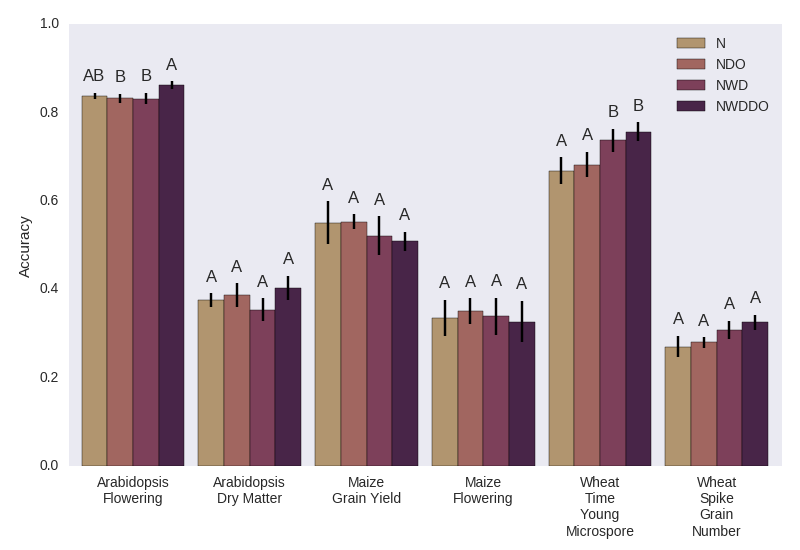
\includegraphics[width=\linewidth]{g3_article/figures/network_comparison.png}
    \caption{Predictive accuracy ($\mu \pm \sigma_{\bar{x}}$) of 
             regularized and non-regularized 
             neural network models for on benchmark datasets. Only the best performing
             network archetecture for each species, trait, and model is included. 
             The accuracy of the best performing model across all folds of data 
             and training cycles were recorded and compared. All pairwise model 
             comparisons within a species and trait were made using a two-sided paired t-test 
             (n=10, paired by training cycle and fold number).
             The resulting p-values were corrected for multiple comparisons within each 
             species and trait combination using the Holm-Bonferroni method. Columns annotated 
             with the same letter are not significantly different 
             at the $\alpha=0.05$ level.}
\label{fig:network-comparison}
\end{figure}
 % Label = fig:network-comparison
\fi

\subsection*{Deep Network Performance}

\ifdefined\showtablesandfigures

\begin{figure}[htbp]
\renewcommand{\familydefault}{\sfdefault}\normalfont
\centering 
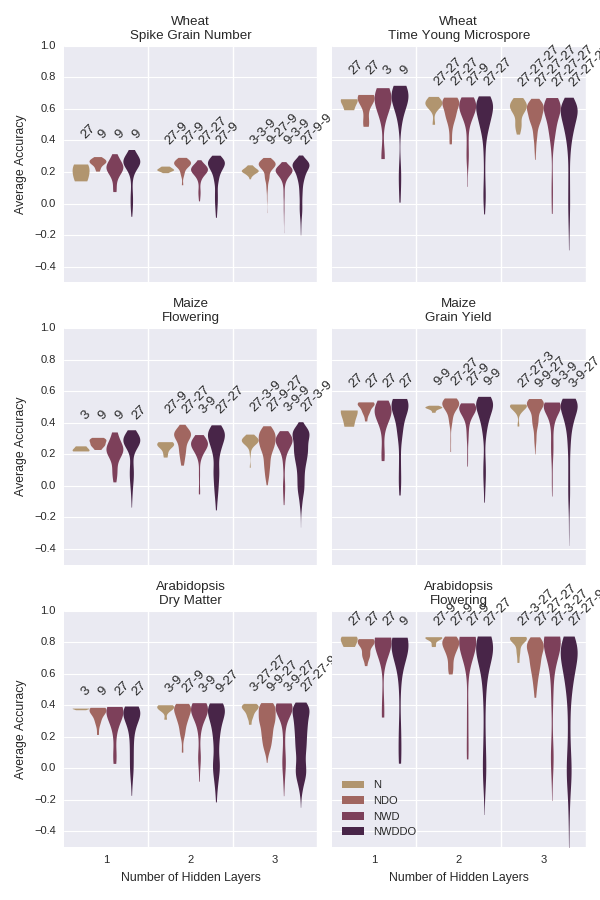
\includegraphics[keepaspectratio,height=\textheight,width=\linewidth]{g3_article/figures/depth_comparison.png}
    \caption{Distribution of predictive accuracy by benchmark dataset, network depth, 
             and model. The violin plot width indicates the Kernel Density Estimate 
             (KDE) of all observed accuracies of all models at a given network depth. 
             The sample size of the KDE is 7, 28, 28, and 112 samples for the 
             N, NWD, NDO, and NWDDO models, respectively. The models contributing 
             to each KDE vary across one or more of five weight decay, five dropout, 
             and seven hidden layer architecture parameters and can be 
             understood as the distribution of results across the set of 
             hyper-parameters to all network models with the same depth and regularization
             type. The KDE bandwidth parameters are set using Scott's normal reference rule. 
             The KDE plots are truncated to the minimum and maximum observed prediction accuracies.} 
\label{fig:depth-comparison}
\end{figure}

 % Label = fig:depth-comparison
\fi

\subsection*{GPU and CPU Training Time}

Network training time was significantly different from CPU training time in all datasets (Figure \ref{fig:time-comparison}).
For small networks trained on smaller datasets such as arabidopsis, CPU training completed significantly faster than GPU training, though only
by a small magnitude. For small networks and all other datasets, as well as for all large networks, GPU training time was faster than 
CPU training time on a per-core basis. For very large datasets such as the pig and loblolly datasets, CPU computing could not be 
completed in under 24 hours, but could be completed by a dedicated GPU card during that time. These results confirm that the 
speedups associated with GPU network training apply to genomic selection applications.  

The results from Figure \ref{fig:time-comparison} compare a single Intel i7-4790K CPU core to a single Nvidia GTX 680 graphics card.
However, most modern full-size computers posess multiple CPU cores, but few contain graphics cards with GPU compute capability. 
Thus, choosing a network training method depends on computing hardware availability as well as required turnaround time. Cloud providers such 
as Amazon Web Services (AWS) are becoming more popular, and make this choice somewhat less important. AWS provides both CPU and GPU rich 
machines which can be rented at low cost and are charged by the hour. This makes it feasible to choose a training platform 
that is most cost effective based on the quantity of data and desired network archetecture for any genomic selection application.

\ifdefined\showtablesandfigures

\begin{figure}[htbp]
\renewcommand{\familydefault}{\sfdefault}\normalfont
\centering 
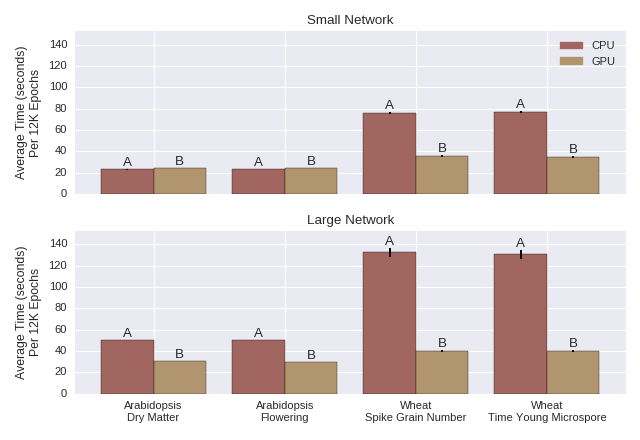
\includegraphics[keepaspectratio,width=\linewidth,height=\textheight]{g3_article/figures/time_comparison.png}
    \caption{Time to train different sized networks on identical datsets using a single dedicated CPU core
             compared to a single dedicated GPU card. Lower time to train is better. For the small network, 
             an unregularized, single hidden layer of 27 neurons was trained for 12K epochs on each dataset. 
             For the large network, two the hidden layers of size 64 and 32 neurons, respectively were trained. 
             Training processes were otherwise equal. This process was repeated ten times per dataset to 
             reduce variation associated with non-deterministic processor scheduling and varying computer system load.
             The ten CPU and GPU training samples were compared using an independent samples T-test with $n=30$. 
             CPU-GPU pairs annotated with the same letter are not significantly different 
             at the $\alpha=0.05$ level.}
\label{fig:time-comparison}
\end{figure}
 % Label = fig:time-comparison
\fi

%\section*{Additional guidelines}
%
%    \subsection*{Numbers} In the text, write out numbers nine or less except as part of a date, a fraction or decimal, 
%                          a percentage, or a unit of measurement. Use Arabic numbers for those larger than nine, 
%                          except as the first word of a sentence; however, try to avoid starting a sentence with such a number.
%
%    \subsection*{Units} Use abbreviations of the customary units of measurement only when they are preceded by a number: 
%            "3 min" but "several minutes". Write "percent" as one word, except when used with a number: 
%            "several percent" but "75\%." To indicate temperature in centigrade, use ° 
%            (for example, 37°); include a letter after the degree symbol only when some 
%            other scale is intended (for example, 45°K).
%
%    \subsection*{Nomenclature and Italicization} Italicize names of organisms even when  when the species is 
%        not indicated.  Italicize the first three letters of the names of restriction enzyme cleavage 
%        sites, as in HindIII. Write the names of strains in roman except when incorporating 
%        specific genotypic designations. Italicize genotype names and symbols, including all components 
%        of alleles, but not when the name of a gene is the same as the name of 
%        an enzyme. Do not use "+" to indicate wild type. Carefully distinguish between genotype 
%        (italicized) and phenotype (not italicized) in both the writing and the symbolism.
%
%\section*{In-text Citations}
%
%Add citations using the \verb|\citep{}| command, for example \citep{neher2013genealogies} or for multiple citations, \citep{neher2013genealogies, rodelsperger2014characterization}.
%
%For examples of different references, please see the example bibliography file 
%(accessible via the Project menu in the Overleaf editor). This contains examples 
%of articles \citep{neher2013genealogies, rodelsperger2014characterization}, a 
%book \citep{Sturtevent2001}, a book 
%chapter 
%XXXX-SKIPPED-XXXX
%%\citep{Sturtevent2001chp7}
%, ahead-of-print work \citep{Starita2015} and software \citep{Kruijer2015}.
%
%\section*{Examples of Article Components}
%\label{sec:examples}
%
%The sections below show examples of different header levels, which you can use in the primary sections of the manuscript (Results, Discussion, etc.) to organize your content.
%
%\section*{First level section header}
%
%Use this level to group two or more closely related headings in a long article.
%
%\subsection*{Second level section header}
%
%Second level section text.
%
%\subsubsection*{Third level section header:}
%
%Third level section text. These headings may be numbered, but only when the numbers must be cited in the text. 
%
%\section*{Figures and Tables}
%
%Figures and Tables should be labelled and referenced in the standard way using the \verb|\label{}| and \verb|\ref{}| commands.
%
%\subsection*{Sample Figure}
%
%Figure \ref{fig:spectrum} shows an example figure.
%
%\begin{figure}[htbp]
%\renewcommand{\familydefault}{\sfdefault}\normalfont
%\centering
%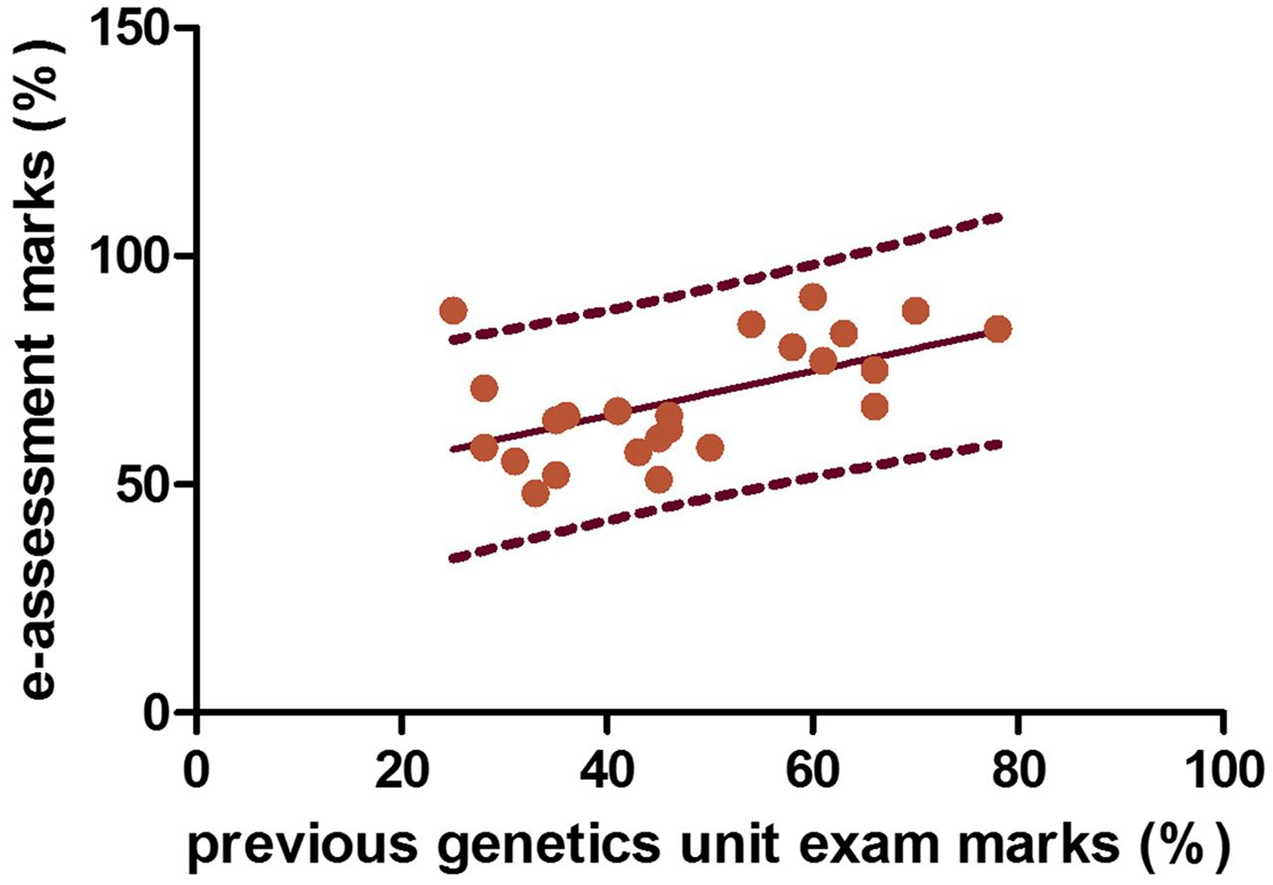
\includegraphics[width=\linewidth]{images/example-figure-g3}
%\caption{Example figure from \url{http://dx.doi.org/10.1534/g3.115.017509}. Please include your figures in the 
%    manuscript for the review process. You can upload figures to Overleaf via the Project menu. Upon acceptance, 
%    we'll ask for your figure files to be uploaded in any of the following formats: TIFF (.tiff), JPEG (.jpg), 
%    Microsoft PowerPoint (.ppt), EPS (.eps), or Adobe Illustrator (.ai).  Images should be a minimum of 
%    300 dpi in resolution and 500 dpi minimum if line art images.  RGB, CMYK, and Grayscale are all 
%    acceptable. Halftones should be high contrast with sharp detail, because some loss of detail and 
%    contrast is inevitable in the production process. Figures should be 10-20 cm in width and 1-25 cm 
%    in height. Graph axes must be exactly perpendicular and all lines of equal density.  Label 
%    multiple figure parts with A, B, etc. in bolded type, and use Arrows and numbers to draw attention 
%    to areas you want to highlight. Legends should start with a brief title and should be a 
%    self-contained description of the content of the figure that provides enough detail to fully 
%    understand the data presented. All conventional symbols used to indicate figure data points are 
%    available for typesetting; unconventional symbols should not be used. Italicize all mathematical 
%    variables (both in the figure legend and figure) , genotypes, and additional symbols that 
%    are normally italicized.  
%}%
%\label{fig:spectrum}
%\end{figure}
%
%\subsection*{Sample Video}
%
%Figure \ref{video:spectrum} shows how to include a video in your manuscript.
%
%\begin{figure}[htbp]
%\renewcommand{\familydefault}{\sfdefault}\normalfont
%\centering
%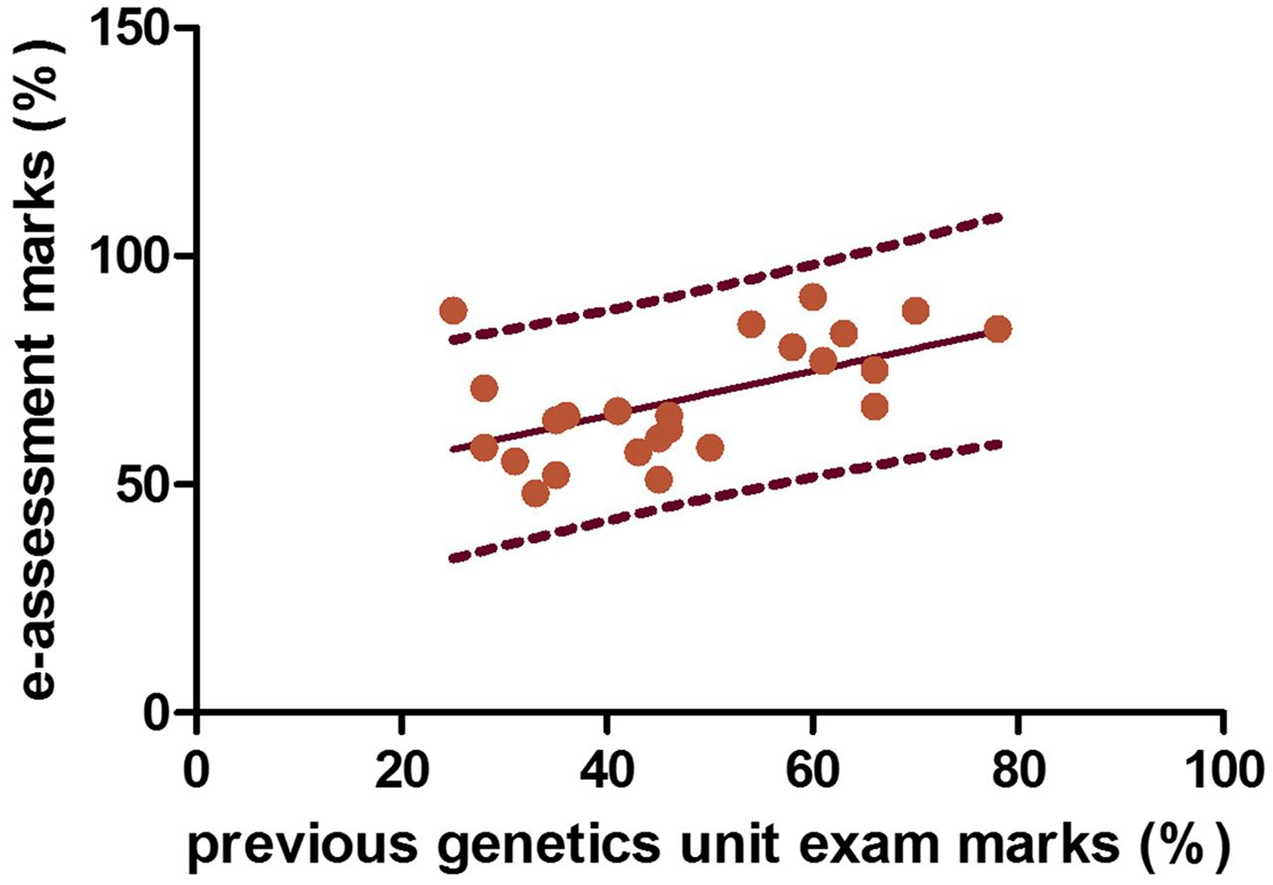
\includegraphics[width=\linewidth]{images/example-figure-g3}
%\caption{Example movie (the figure file above is used as a placeholder for this example). G3 supports video and movie 
%         files that can be linked from any portion of the article - including the abstract. Acceptable formats include 
%         .asf, avi, .wav, and all types of Windows Media files.   
%}%
%
%\label{video:spectrum}
%\end{figure}
%
%
%\subsection*{Sample Table}
%
%Table \ref{tab:shape-functions} shows an example table. Avoid shading, color type, line drawings, graphics, or 
%                                other illustrations within tables. Use tables for data only; present drawings, graphics, 
%                                and illustrations as separate figures. Histograms should not be used to present data 
%                                that can be captured easily in text or small tables, as they take up much more space.  
%
%Tables numbers are given in Arabic numerals. Tables should not be numbered 1A, 1B, etc., but if necessary, 
%interior parts of the table can be labeled A, B, etc. for easy reference in the text.  


%\begin{table*}[htbp]
%\renewcommand{\familydefault}{\sfdefault}\normalfont
%\centering
%\caption{\bf Students and their grades}
%\begin{tableminipage}{\textwidth}
%\begin{tabularx}{\textwidth}{XXXX}
%\hline
%\header Student & Grade\footnote{This is an example of a footnote in a table. Lowercase, superscript italic letters (a, b, c, etc.) are used by default. You can also use *, **, and *** to indicate conventional levels of statistical significance, explained below the table.} & Rank & Notes \\
%\hline
%Alice & 82\% & 1 & Performed very well.\\
%Bob & 65\% & 3 & Not up to his usual standard.\\
%Charlie & 73\% & 2 & A good attempt.\\
%\hline
%\end{tabularx}
%  \label{tab:shape-functions}
%\end{tableminipage}
%\end{table*}

%\section*{Sample Equation}
%
%Let $X_1, X_2, \ldots, X_n$ be a sequence of independent and identically distributed random variables with $\text{E}[X_i] = \mu$ and $\text{Var}[X_i] = \sigma^2 < \infty$, and let
%\begin{equation}
%S_n = \frac{X_1 + X_2 + \cdots + X_n}{n}
%      = \frac{1}{n}\sum_{i}^{n} X_i
%\label{eq:refname1}
%\end{equation}
%denote their mean. Then as $n$ approaches infinity, the random variables $\sqrt{n}(S_n - \mu)$ converge in distribution to a normal $\mathcal{N}(0, \sigma^2)$.


\bibliography{bibliography}

\end{document}
